\section{Background and Motivations}
Failures(e.g., process crash, kernel panics, power outages) are common in systems like Database systems and File systems, even in robust enough Distributed systems, which will incur fatal problems such as inconsistency and data loss. Techniques have been proposed to address these issues, for example, systems offten leverage Log and Replication to handle failures. In this paper, we focus on Log especially write-ahead log, systems will log changes into Log for persistency, then to the real place,  When restarting, systems recovery from Log take advantage of full operation informations in Log.

But the logging when forward processing and recovery from Log after failures are both too slow to support high-level application well, which is intolerable even for a single node. the architeture and process flow of a single node is illustrated as Fig.~\ref{fig:architecture}. The \texttt{Disk} and \texttt{Dram} are managed by page. When transactions want to operate, they map the operations into Data buffer in step 1, then log the operations in Log buffer in step 2, the log entries in Log buffer will be flushed to durable storage for persistency in step 3, then, if the flush returns successfully in step 4, the system will inform user that the operations are completed, and the system will flush the dirty page in Data buffer into durable storage later in step 5.

Generally, systems leverage single Log to log and recover for simple, this is why the logging and revovery are so slow. First, the multiple threads will contend to write to a single Log, second, a sequential scan will be performed over the corresponding log by only one thread. Both of them will cause worse scalability as the number of threads grows in a single node with multi-core.

A straightforward approach to speed up the logging and recovery is distributing the Log, for example, one Log file per processor. But the distributed Log is still tardy because of too many cross-log dependencies.

In this paper, we propose a new version of distributed Log by leveraging a few techniques, which will support parallelism well in single node with multi-core.
% Modern distributed file systems, such as GFS\cite{ghemawat2003google}, HDFS\cite{shvachko2010hadoop}, Ceph\cite{weil2006ceph}, which consist of three components, metadata servers(MDS), object-based storage devices(OSD) and clients as Fig.~\ref{fig:architecture} shows. Clients perform metadata operations(\emph{open, stat}) directly with MDS and file I/O directly with data server. This architecture decouples metadata I/O from data IO and increases overall scalability. For example, client requests data with pathname /var/log/client.log. By multiple interactions to MDS, client lookups the directory of \texttt{root}, \texttt{var} and \texttt{log} to locate the inode of \texttt{client.log} and checks the permission. Once client obtain the inode, it must get the capability to access to data. Then, client will request a lease on this file to MDS. Finnaly, client interact with OSD to operator file I/O. Due to the iterative lookup and checking permission operations, the IOs between clients and MDS are more than OSD. Because overall 50\% of IOs are to metadata\cite{roselli2000comparison}, metadata performance is crucial.

% \begin{figure}[htbp]
%   \centering
%   % Requires \usepackage{graphicx}
%   %\vspace{-5pt}
%   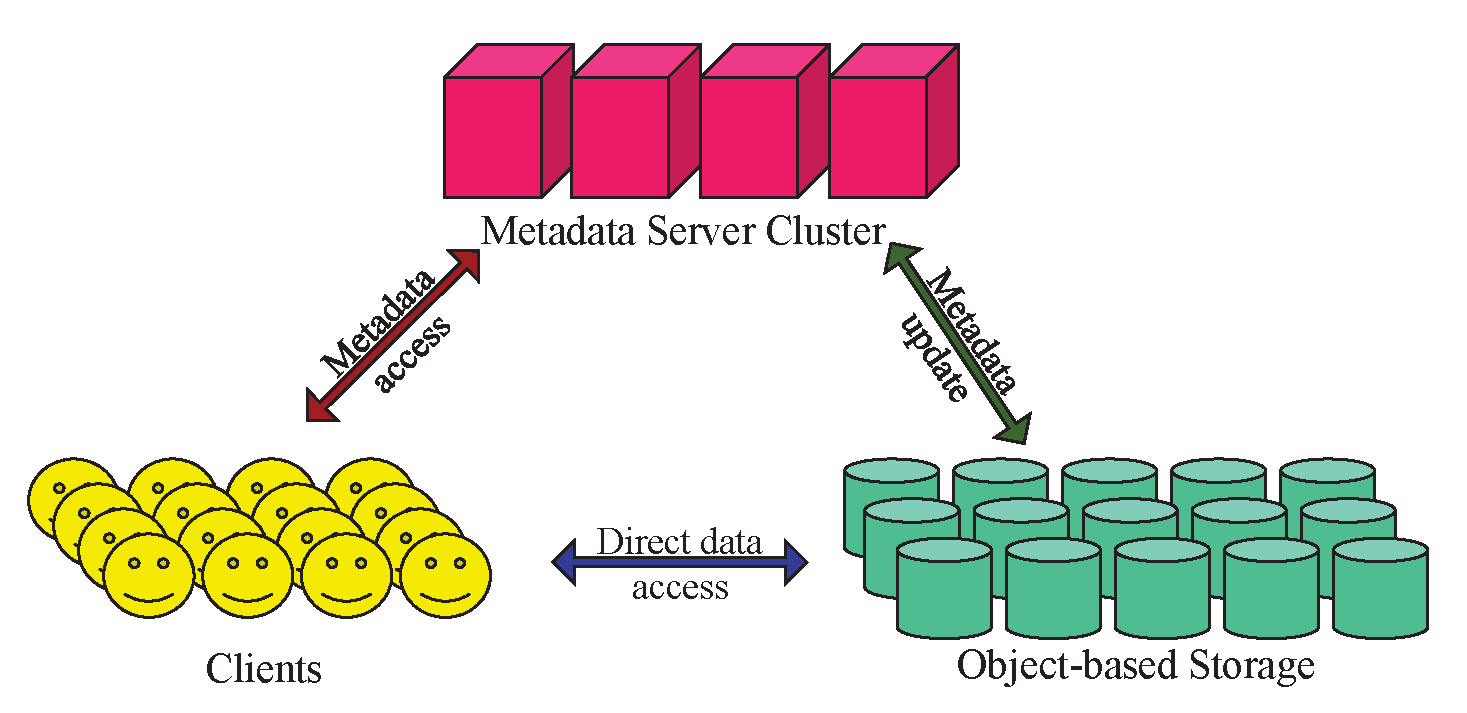
\includegraphics[width=1\linewidth]{architecture.eps}\\
%   %\vspace{-10pt}
%   \caption{Architecture of distributed file systems.}\label{fig:architecture}
%    %\vspace{-10pt}
% \end{figure}
\begin{figure}[htbp]
  \centering
  % Requires \usepackage{graphicx}
  %\vspace{-5pt}
  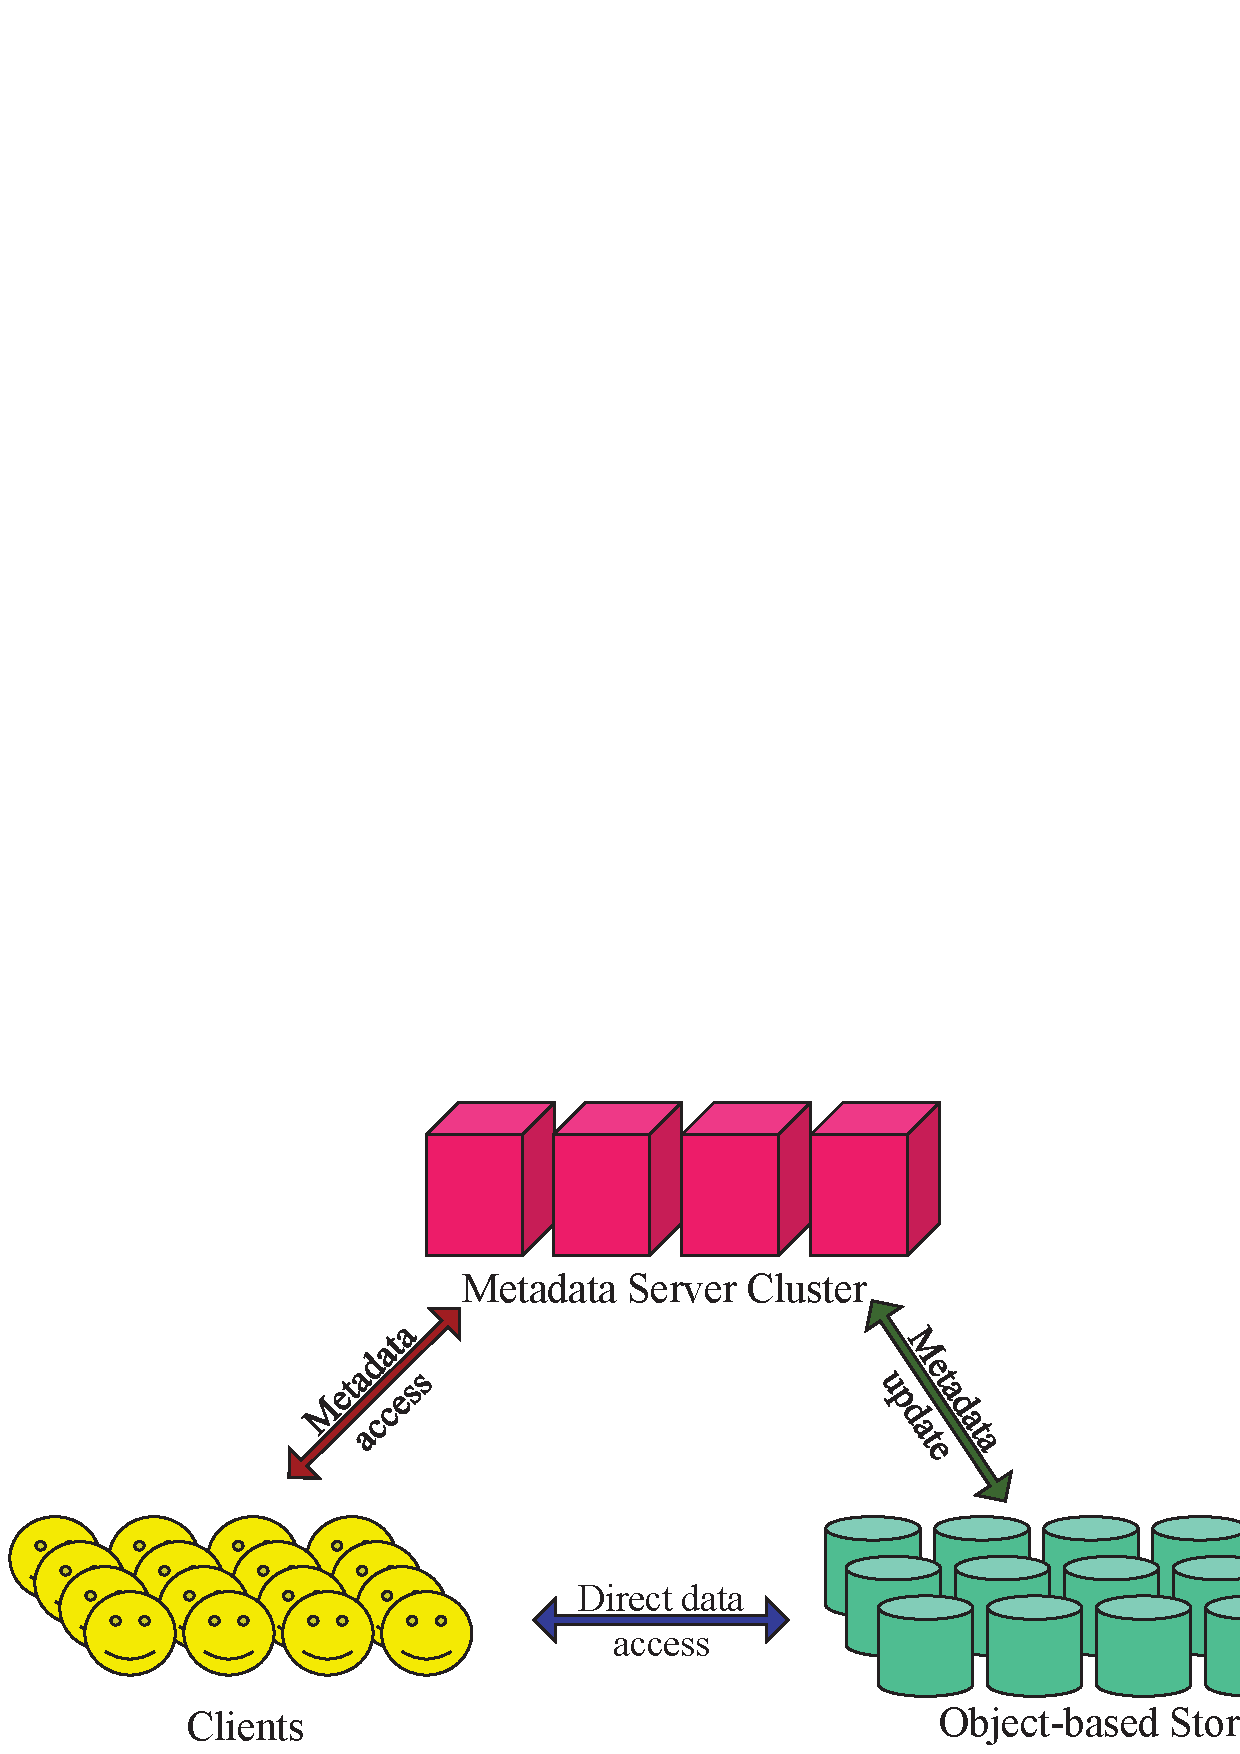
\includegraphics[width=1\linewidth]{architecture.jpg}\\
  %\vspace{-10pt}
  \caption{Architecture and process flow of write-ahead logging.}\label{fig:architecture}
   %\vspace{-10pt}
\end{figure}


% In this paper, we propose a correlations-based metadata prefetching to reduce IO traffic to MDS, to scale distributed file systems, to increase client cache hit ratio with high accuracy and low false positive. How to define the correlations among files and how to update correlations in real time become a challenge.
